\section{Model and open loop analysis}
\subsection{Model analysis}
The continue state space model where $u=V$ (voltage on the motor) and x=$[\theta \ \alpha \  \dot{\theta} \ \dot{\alpha} ]$ is theoretical derived in the assignment and leads to the following system. The system can only directly measure $\theta$ and $\alpha$, so these determine the matrix C and D.

$$
\begin{cases}
\dot{x}=Ax+Bu \\
y=Cx+Du
\end{cases}
$$

$$
A=
\begin{bmatrix}
0 & 0 & 1 & 0 \\
0 & 0 & 0 & 1 \\
0 & 40.7 & -12.2 & 0 \\
0 & 38.6 & -4.7 & 0 
\end{bmatrix}
B=
\begin{bmatrix}
0 \\
0 \\
23.3 \\
8.3
\end{bmatrix}
C=
\begin{bmatrix}
1 & 0 & 0 & 0\\
0 & 1 & 0 & 0
\end{bmatrix}
D=
\begin{bmatrix}
0 & 0
\end{bmatrix}
$$

\subsection{Open loop analysis}

The system contains 1 unstable pole at about 5.3 (see figure~\ref{fig:zplot system}), this obviously means that the system is unstable. The rank of the controllability matrix is 4, the smallest singular value of the controllability matrix is 1.7. So the system is controllable, which is very useful if its of an unstable nature. The observability matrix is of rank 4 which with a smallest singular value of 1. So the system is observable.
%M: Ik zou niet zeggen dat het erg handig is dat een onstabiel systeem contolable is, het is nuttig dat een systeem controlable is waneer je het wilt controleren en het is voldoende als je een onstabiel systeem wilt stabilizeren dat het stabilizeerbaar is. Maar de zin die er nu staat vind ik wat veermd, niet?

\begin{figure}[H]
	\centering
	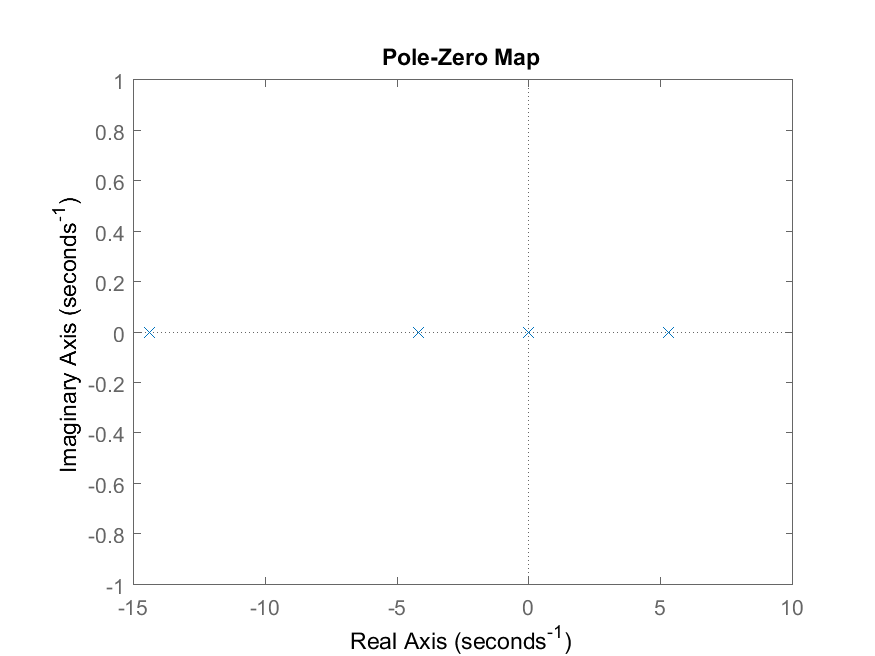
\includegraphics[width=0.5\textwidth]{./part1_analysis/zplot.png}
	\caption{plot of poles and zeros}
	\label{fig:zplot system}
\end{figure}

If the system is controllable then it's stabilizable and if its observable then it's also detectable which means that if there are unstable states, they you can at least detect unstability.

\subsection{control goals}

Our goals of the controller is to make a stable robust system, it must not be very fast because it will than also be more nervous. We would like that the system can track setpoints up to some step-responses. But our objective is more a robustness system than a fast one.